% Use only LaTeX2e, calling the article.cls class and 12-point type.

\documentclass[12pt]{article}

% Users of the {thebibliography} environment or BibTeX should use the
% scicite.sty package, downloadable from *Science* at
% www.sciencemag.org/about/authors/prep/TeX_help/ .
% This package should properly format in-text
% reference calls and reference-list numbers.

%подключение русского языка
\usepackage{cmap}
\usepackage[T2A]{fontenc}
\usepackage[utf8]{inputenc}
\usepackage[english, russian]{babel}


\usepackage{scicite}

\usepackage{indentfirst} %Красная строка

\usepackage{amsmath} %текст в формулах

\usepackage{graphicx} %графика
\DeclareGraphicsExtensions{.pdf,.png,.jpg}



% Use times if you have the font installed; otherwise, comment out the
% following line.

\usepackage{times}

% The preamble here sets up a lot of new/revised commands and
% environments.  It's annoying, but please do *not* try to strip these
% out into a separate .sty file (which could lead to the loss of some
% information when we convert the file to other formats).  Instead, keep
% them in the preamble of your main LaTeX source file.


% The following parameters seem to provide a reasonable page setup.

\topmargin 0.0cm
\oddsidemargin 0.2cm
\textwidth 16cm 
\textheight 21cm
\footskip 1.0cm


%The next command sets up an environment for the abstract to your paper.

\newenvironment{sciabstract}{%
\begin{quote} \bf}
{\end{quote}}


% If your reference list includes text notes as well as references,
% include the following line; otherwise, comment it out.

\renewcommand\refname{References and Notes}

% The following lines set up an environment for the last note in the
% reference list, which commonly includes acknowledgments of funding,
% help, etc.  It's intended for users of BibTeX or the {thebibliography}
% environment.  Users who are hand-coding their references at the end
% using a list environment such as {enumerate} can simply add another
% item at the end, and it will be numbered automatically.

\newcounter{lastnote}
\newenvironment{scilastnote}{%
\setcounter{lastnote}{\value{enumiv}}%
\addtocounter{lastnote}{+1}%
\begin{list}%
{\arabic{lastnote}.}
{\setlength{\leftmargin}{.22in}}
{\setlength{\labelsep}{.5em}}}
{\end{list}}


% Include your paper's title here


\title{Определение $C_{v}$/$C_{p}$ по скорости звука в газе (2.1.3)} 

% Place the author information here.  Please hand-code the contact
% information and notecalls; do *not* use \footnote commands.  Let the
% author contact information appear immediately below the author names
% as shown.  We would also prefer that you don't change the type-size
% settings shown here.

\author
{Иван Едигарьев,$^{1}$ 526т \\
\\
\normalsize{$^{1}$Факультет Общей и Прикладной Физики,}\\ \normalsize{}{Московский Физико-Технический Институт}\\
}

% Include the date command, but leave its argument blank.

\date{}



%%%%%%%%%%%%%%%%% END OF PREAMBLE %%%%%%%%%%%%%%%%



\begin{document} 

% Double-space the manuscript.

\baselineskip24pt

% Make the title.

\maketitle 



% Place your abstract within the special {sciabstract} environment.

\begin{sciabstract}
Цель работы: 1) измерение частоты колебаний и длины волны при резонансе звуковых колебаний в газе, заполняющем трубу; 2) определение показателя адиабаты с помощью уравнения состояния идеального газа. 

В работе используются: звуковой генератор ГЗ; электронный осциллограф ЭО; микрофон; телефон; раздвижная труба; теплоизолированная труба, обогреваемая водой из термостата; баллон со сжатым углекислым газом; газгольдер. 

\end{sciabstract}



% In setting up this template for *Science* papers, we've used both
% the \section* command and the \paragraph* command for topical
% divisions.  Which you use will of course depend on the type of paper
% you're writing.  Review Articles tend to have displayed headings, for
% which \section* is more appropriate; Research Articles, when they have
% formal topical divisions at all, tend to signal them with bold text
% that runs into the paragraph, for which \paragraph* is the right
% choice.  Either way, use the asterisk (*) modifier, as shown, to
% suppress numbering.

\section*{Теория}

Скорость распространения звуковой волны в газах зависит от показателя адиабаты $\gamma$. На измерении скорости звука основан один из наиболее точных методов определения показателя адиабаты.

Скорость звука в газах определяется формулой:
$$ c = \sqrt{\gamma\frac{RT}{\mu}},$$

где $R$ — газовая постоянная, $T$ — температура газа, а $\mu$ — его молярная масса. 
\newpage
Преобразуя эту формулу, най̆дем
\begin{equation}\label{1}
    \gamma = \frac{\mu}{RT}c^2 
\end{equation}
Таким образом, для определения показателя адиабаты достаточно измерить температуру газа и скорость распространения звука (молярная масса газа предполагается известной).

Звуковая волна, распространяющаяся вдоль трубы, испытывает многократные отражения от торцов. Звуковые колебания в трубе являются наложением всех отраженных волн и, вообще говоря, очень сложны. Картина упрощается, если длина трубы L равна целому числу полуволн, то есть когда
\begin{equation}\label{2}
    L = n\lambda/2
\end{equation}
где $\lambda$ — длина волны звука в трубе, а $n$ — любое целое число. Если условие (\ref{2}) выполнено, то волна, отраженная от торца трубы, вернувшаяся к ее началу и вновь отраженная, совпадает по фазе с падающей. Совпадающие по фазе волны усиливают друг друга. Амплитуда звуковых колебаний при этом резко возрастает — наступает резонанс.

При звуковых колебаниях слои газа, прилегающие к торцам трубы, не испытывают смещения (узел смещения). Узлы смещения повторяются по всей длине трубы через $\lambda/2$. Между узлами находятся максимумы смещения (пучности).

Скорость звука c связана с его частотой $f$ и длиной волны $\lambda$ соотношение
\begin{equation}\label{3}
    c = \lambda{f}
\end{equation}

Подбор условий, при которых возникает резонанс, можно производить двояко:

\newpage

1. При неизменной частоте $f$ звукового генератора (а следовательно, и неизменной длине звуковой волны $\gamma$) можно изменять длину трубы $L$. Для этого применяется раздвижная труба. Длина раздвижной трубы постепенно увеличивается, и наблюдается ряд последовательных резонансов. Возникновение резонанса легко наблюдать на осциллографе по резкому увеличению амплитуды колебаний. Для последовательных резонансов имеем

\begin{align}\notag
    L_n = n\frac{\lambda}{2},\text{     }\text{     }\text{     }
    L_{n+1} = (n+1)\frac{\lambda}{2},\text{     }\text{     }
    \text{      ...,    }\text{     }\text{     }
    L_{n+k} = n\frac{\lambda}{2}+k\frac{\lambda}{2}
\end{align}


т. е. $\lambda/2$ равно угловому коэффициенту графика, изображающего зависимость длины трубы $L$ от номера резонанса $k$. Скорость звука находится по формуле (\ref{3}).

2. При постоянной длине трубы можно изменять частоту звуко- вых колебаний. В этом случае следует плавно изменять частоту $f$ звукового генератора, а следовательно, и длину звуковой волны $\gamma$. Для последовательных резонансов получим

\begin{align}\label{4}
    L = \frac{\lambda_1}{2}n =\frac{\lambda_2}{2}(n+1) = \text{    ...     }=\frac{\lambda_{k+1}}{2}(n+k)
\end{align}

Из (\ref{3}) и (\ref{4}) имеем

\begin{align}\notag
    f_1 = \frac{c}{\lambda_1} = \frac{c}{2L}n, \text{   }\text{   } f_2 = \frac{c}{\lambda_2} = \frac{c}{2L}(n+1) = f_1 + \frac{c}{2L}, \text{     }\text{     }
    \text{      ...,    }\text{     }\text{     }
\end{align}
\begin{align}\label{5}
    f_{k+1} = \frac{c}{\lambda_{k+1}} = \frac{c}{2L}(n+k) = f_1 + \frac{c}{2L}k
\end{align}

Скорость звука, деленная на 2$L$, определяется, таким образом, по угловому коэффициенту графика зависимости частоты от номера резонанса.

\section*{Экспериментальная установка}
Экспериментальная установка. Соответственно двум методам измерения скорости звука в работе имеются две установки (рис. 1 и 2). В обеих установках звуковые колебания в трубе возбуждаются телефоном $T$ и улавливаются микрофоном $M$. Мембрана телефона приводится в движение переменным током звуковой частоты; в качестве источника переменной ЭДС используется звуковой генератор ГЗ. Возникающий в микрофоне сигнал наблюдается на осциллографе Э$0$.

Микрофон и телефон присоединены к установке через тонкие резиновые трубки. Такая связь достаточна для возбуждения и обнаружения звуковых колебаний в трубе и в то же время мало возмущает эти колебания: при расчетах оба торца трубы можно считать непоlвижными, а влиянием соединительных отверстий пренебречь.

Первая установка (рис. 1) содержит раздвижную трубу с миллиметровой шкалой. Через патрубок (на рисунке не показан) труба может наполняться воздухом или углекислым газом из газгольдера. На этой установке производятся измерения γ для воздуха и для $CO2$. Вторая установка (рис. 2) содержит теплоизолированную трубу поcтоянной длины. Воздух в трубе нагревается водой из термостата. Температура газа принимается равной температуре омывающей трубу воды. На этой установке измеряется зависимость скорости звука от температуры.

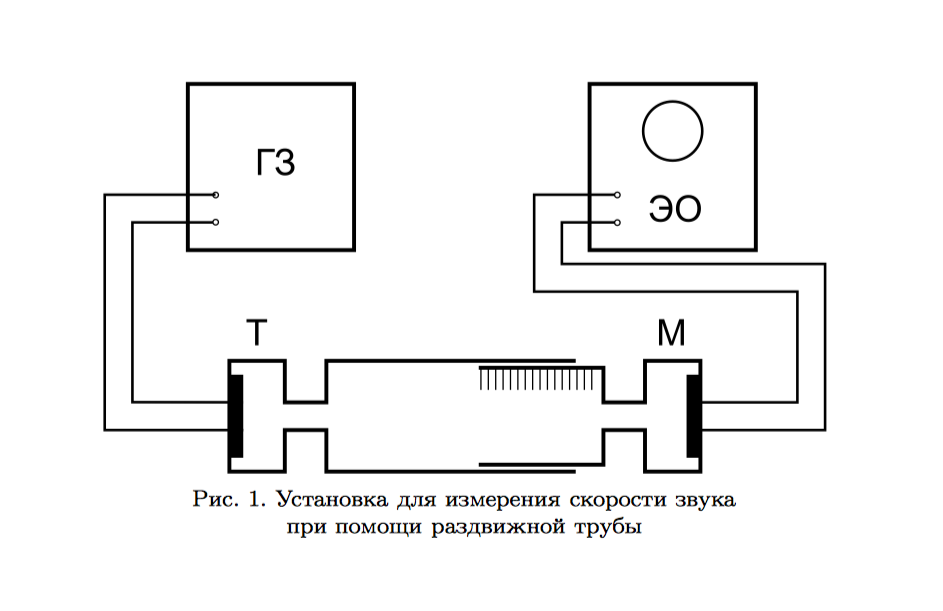
\includegraphics[scale = 0.46]{gr1} \\
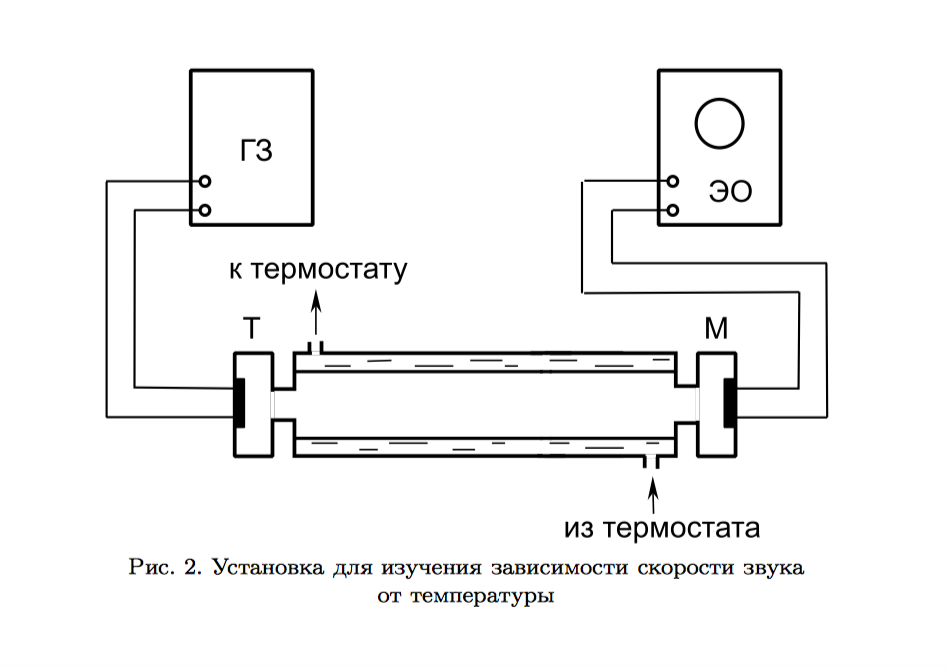
\includegraphics[scale = 0.46]{gr2}
\section*{Ход работы и задание}

1. Включите в сеть электронный осциллограф Э$0$ и звуковой генератор ГЗ и дай̆те им прогреться 5–7 минут. После этого включите тумблер «Луч» и ручками управления осциллографа добейтесь того, чтобы на экране была видна линия, прочерченная электронным лучом.

Установите нулевое значение шкалы частот звукового генератора (только для генератора ГЗ-18). Для этого лимбы «Частота» и «Расcтройка» установите на нуль и вращением ручки «Установка нуля» добейтесь того, чтобы стрелка вольтметра остановилась на нуле. Время от времени проверяйте, не сбилась ли установка нуля.

2. Подберите напряжение на выходе генератора так, чтобы при резонанce на осциллографе наблюдались колебания достаточной амплитуды. Остановите картину на осциллографе. Убедитесь в том, что колебания имеют неискаженную синусоидальную форму. Если форма колебаний искажена, уменьшайте амплитуду сигнала, поступающего с генератора, пока искажения не прекратятся.

3. Измерения на первой установке (рис. 1).

а) Исходя из примерного значения скорости звука (300 м/с), рассчитайте, в каком диапазоне частот следует вести измерения, чтобы при удлинении трубы можно было наблюдать 2–5 резонансов.

б) Используя многоходовый или кнопочный кран, продуйте трубу воздухом (в ней мог остаться углекислый газ). Плавно изменяя длину трубы, последовательно пройдите через все доступные для наблюдения точки резонанса. Повторите измерения при других частотах (всего 4–6 различных значений частоты). Для каждого резонанса измерьте соответствующее удлинение трубы. Проведите измерения,сначала увеличивая длину трубы, а затем уменьшая ее.

в) Изобразите полученные результаты на графике, откладывая по оси абсцисс номер $k$ последовательного резонанса, а по оси ординат — соответствующее удлинение трубы $L_n+k$ − $L_n$. Через точки, полученные при одном и том же значении частоты, проведите наилучшую прямую. Угловой коэффициент прямой определяет длинуполуволны.

По графику оцените ошибку измерения $\lambda/2$. Вычислите значение скорости звука и оцените точность полученного результата. (Ошибка в градуировке шкалы частот генератора не превосходит половины минимального деления шкалы.) Сопоставьте значения скорости звука, измеренные на разных частотах. Находятся ли эти значения в согласии друг с другом? Найдите наилучшее значение скорости звука, используя все результаты измерений.

г) Измерьте скорость звука в углекислом газе. Перед началом измерений продуйте трубу углекислым газом. Для этого при открытом кране подвижную часть трубы следует несколько раз медленно выдвинуть и затем резко вдвинуть в трубу. Температура газа равна комнатной. Измерять резонансные максимумы нужно при открытом кране $CO2$ и при медленных перемещениях подвижной части трубы как внутрь, так и наружу.

По окончании этих измерений подвижную часть трубы оставьте во вставленном состоянии и проведите измерения резонансных макcимумов при увеличении и затем при уменьшении частоты. Обработайте полученные данные и сравните результаты с полученными при изменении длины трубы.

4. Измерения на второй установке (рис. 2).

а) Измерьте скорость звука в трубе постоянной длины. Плавноувеличивая частоту генератора, получите ряд последовательных резонансных значений частоты, отмечая момент резонанса по увеличению амплитуды колебаний на экране осциллографа. Убедитесь в повторяемости результатов, производя измерения при уменьшении частоты.

б) Полученные результаты изобразите на графике, откладывая по оси абсцисс номер резонанса $k$, а по оси ординат — разность между частотой последующих резонансов и частотой первого резонанса: $f_{k+1} - f_1$. Через полученные точки проведите наилучшую прямую. Угловой коэффициент прямой определяет величинy $c/2L$ (\ref{5}). Вычислите значение скорости звука. Оцените ошибку измерений.


в) Включите термостат. Повторите измерения пп. а) и б) еще при трех значениях температуры в интервале от комнатной до $80^\circ$C. Найдите скорость звука при каждом выбранном значении температуры.

5. Вычислите значение $\gamma = C_p/C_v$ по формуле (\ref{1}). Оцените ошибку измерений̆.

\newpage

\section*{Измерения}

\bibliography{scibib}
\bibliographystyle{Science}

\end{document}




















